\documentclass{article}
\usepackage[utf8]{inputenc}
\usepackage{biblatex}
\usepackage{graphicx}
\usepackage{placeins}
\usepackage{algorithm}
\usepackage{algpseudocode}
\usepackage[font={small}]{caption}
\usepackage{minted}
\usepackage{float}
\usepackage{placeins}
\usepackage{url}
\usepackage[margin=1in]{geometry}
\usepackage{array, caption, tabularx, ragged2e, booktabs}
\usepackage[toc, page]{appendix}

\def\UrlBreaks{\do\/}

\algdef{SE}[DOWHILE]{Do}{doWhile}{\algorithmicdo}[1]{\algorithmicwhile\ #1}%

\makeatletter
\def\BState{\State\hskip-\ALG@thistlm}
\makeatother

\addbibresource{sources.bib}

\title{Scheduling in Clouds: A deep analysis of different allocation policies}
\author{
    Willemijn Beks, Kaan Kara, Daan Kruis, Sander Ronde, Mike Schouw \\
    \texttt{\{j.w.z.beks, h.k.kara, d.kruis, s.j.p.m.ronde, m.j.schouw\}@student.vu.nl}
    % \\ \small 2669090
    % \and 
    %  \\ \small 2635400
    % \and
    %  \\ \small 2545363
    % \and
    %  \\ \small 2639938
    % \and
    %  \\ \small 2655677
}
\date{December 2019}

\begin{document}

\maketitle

\begin{abstract}
This paper describes the implementation and comparing of Fast Critical Path scheduling, Lottery scheduling, and Delay scheduling with help of the OpenDC framework. They are tested on three different workflows and with homogeneous and heterogeneous setups. The three algorithms performed similarly, with Delay Scheduling outperforming the other two on the smallest and most heterogeneous workflow.
\end{abstract}

\section{Introduction}
Scheduling workflows in large datacentres can be done in different ways with different scheduling techniques that all have their own characteristics. These characteristics decide how scheduling is done. A scheduling policy can be (among others) greedy or heuristic, it can base its decisions on cost, makespan or fairness and scheduling can be done offline or online. The cloud computing market is a very big market and expanding still, with more clients every day.\\
All those different clients mean different goals and lots of money being spend to make sure those goals can be met. This means that optimizing and improving functionalities in the cloud, means earning potentially lots of money and satisfying more customers. This means that making an informed choice on which schedulers to choose is important as they are a vital part of the functioning of the cloud. \\
In this paper we present three different existing allocation policies that we have implemented and tested with the use of OpenDC, comparing their performance on different workflows. We compare Fast Critical Path (FCP), Delay Scheduling, and Lottery scheduling. All the algorithms we compared are offline since the workflows that were available had all the necessary information to schedule at compile time. The Fast Critcial Path algorithm is a heuristic algorithm that uses timestamps that tries to minimize makespan, delay Scheduling uses fairness and cost and lottery scheduling is mostly fair since it is an almost random scheduling technique. Our implementation provides insight into the performance of different offline schedulers. It is expected that FCP and Delay Scheduling will outperform Lottery Scheduling since algorithms that use some approach to optimize performance should in theory be better than random most of the time. We expect delay scheduling to have the best performance if it is given a workload with many dependencies, if not, Fast Critical Path will likely be the best performing algorithm.
For workflows we used three different ones, where we test homogeneous and heterogeneous jobs, on moderately sized workflows. 
\\
Section 3 describes the algorithms that are used for our experiments, their characteristics, trade-offs and implementation. Section 4 contains the setup of our experiments. Section 5 contains the results of our experiments in the previously stated section. Section 6 describes the conclusions found in our experiments. This paper ends with the last section, Section 7, containing our discussion.    


\section{Algorithms}
Our fork of the opendc-simulator repository can be found at \cite{OpenDC-fork}. It contains the algorithms discussed below as well as this report and its source code. The algorithms FCP, Delay Scheduling and Lottery Scheduling can be found in the fork's $Selection.kt$ file~\cite{algo-file}. The schedulers will be added to the main OpenDC repository shortly via pull requests.

\subsection{Fast Critical Path}
\subsubsection{Overview}
Fast Critical Path Algorithm is a scheduling algorithm which uses timestamps as heuristic. In the paper about FCP \cite{Radulescu99onthe}, it is argued that list scheduling algorithms perform better on systems with a limited number of processors. Even though the performance of list scheduling algorithms is better, it is argued that their complexity is much higher than multi-step scheduling. The rationale behind FCP is to decrease its complexity while keeping the performance gains, for example sorting tasks based on their priority has \textit{O(VlogV)} complexity, and in theory, not sorting all the task list will decrease the complexity. In-depth complexity analysis of FCP algorithm can be found in \cite{Radulescu99onthe}. The main point of FCP is to decrease the complexity of list scheduling algorithms while keeping their benefits. From the theoretical perspective, it decreases the complexity of the algorithm, but the practical outcome of the algorithm will be shown in Section \ref{experiments}.
\subsubsection{Approach}
FCP tries to optimize the makespan time of a task using processor timestamps, meaning it uses a heuristic approach to solve the problem at hand. Based on the timestamps, it either reduces communication overhead by choosing the processor that the last message is received from or tries to ensure processor load balancing by considering the earliest processor to become idle. The best processors in list scheduling algorithms are the ones where the task to be scheduled starts earliest \cite{Radulescu99onthe}. Based on this assumption, one of the candidates that has the earliest starting time is selected. FCP does not use any advanced heuristics, thus it is not able to take advantage of any kind of workflows. It is expected FCP to perform worst at locality and data-intensive workflows.
\subsubsection{Trade-Offs}
FCP is relatively the easiest algorithm to implement among all three algorithms chosen in this experiment. It can take priorities into account; however, it does not sort the list of all tasks, it rather sorts only a fixed sub list of the list of all tasks. This implies that the task with the highest priority is not guaranteed to be run always. On the other hand, ordered sub list approach prevents task starvation, meaning the priority of a task cannot be abused, and other tasks will eventually be run without waiting on the task with highest priority until it terminates.
FCP works at processor granularity, so it needs a notion of unified system, and it needs modifications to be able to work with tasks that require multiple processors. In modern distributed systems, instead of using processor granularity, machine granularity is used as it is used in OpenDC. This approach also enables the use of locality where FCP is not interested in this matter at all, therefore this algorithm can work well with processor intensive tasks, but multi-processor data intensive tasks are not expected to work well on this algorithm.
FCP considers two candidate processors to schedule the task on. This is done to reduce the complexity of choosing a processor by scanning whole processor graph. It is argued that a given task cannot start earlier on any other processors \cite{Radulescu99onthe}. In this part, FCP manages to decrease the complexity of processor selection without any performance impact on the algorithm.
\subsubsection{Implementation}
FCP algorithm consists of 3 main routines; AddReadyTask, SelectReadyTask, and SelectProcessor. The algorithm keeps tasks in two separate lists which are a fixed size ordered list and an unordered list. Overview of FCP algorithm can be seen in Algorithm \ref{fcp-algorithm}. AddReadyTask, adds runnable tasks to the sorted list. In OpenDC implementation of this algorithm, AddReadyTask routine is omitted since Task Filtering does filter runnable tasks and pass the list of runnable tasks to Sorting Policy. The next part of the algorithm is SelectReadTask. SelectReadyTask, basically selects a runnable task from the ordered list. In OpenDC implementation, the runnable task list -which was passed from AddReadyTask stage of the algorithm- is partially sorted and a task is popped from it. 
SelectProcessor routine selects a suitable processor. It evaluates 2 candidates based on their timestamps. The first candidate is the processor that has become idle the earliest, and the second candidate is the one that the last message is received from. OpenDC works at machine granularity, so implementing this part of the algorithm directly is not possible. OpenDC implementation of this routine instead uses machines’ timestamps. 

\begin{algorithm}[H]
\caption{Fast Critical Path}\label{fcp-algorithm}
\begin{algorithmic}[1]
\For {t $\in$ V} 
\State $\textit{ComputePriority(t)}$
\If {t is an entry task} 
\State $\textit{AddReadyTask(t)}$
\EndIf
\EndFor
\While {$\textbf{NOT}$ all tasks scheduled}
\State $\textit{task} \gets$ $\textit{SelectReadyTask()}$ 
\State $\textit{p} \gets$ $\textit{SelectProcessor(task)}$
\State $\textit{ScheduleTask(Task, p)}$
\For {t $\in$ new ready task set}
\State $\textit{AddReadyTask(t)}$
\EndFor
\EndWhile
\end{algorithmic}
\end{algorithm}


\subsection{Delay Scheduling}
\subsubsection{Overview}
Delay scheduling is an allocation policy created by Zaharia, Matei, et al. \cite{zaharia2010delay}. The goal of this allocation policy is to achieve near optimal data locality, the placement of computation near its input data, while also preserving fairness. 
\subsubsection{Approach}
Delay scheduling does not use preemption to achieve fairness and data locality, instead it does quite the opposite, it waits. Killing tasks to schedule newly arrived tasks has a big disadvantage since all the work of task is lost. However, waiting for a task to be scheduled on the machine of its predecessors may also decrease fairness, since this could take a lot of time. The algorithm copes with this by scheduling the skipped tasks eventually, even if the desired machine is not available. With regards almost optimal data locality, the shows that a very small amount of waiting is enough to bring locality close to 100{\%} \cite{zaharia2010delay}.

\subsubsection{Trade-Offs}
The disadvantage of this scheduling policy is that it only works well when the workload consists of tasks with many dependencies. Only then, the tasks can get scheduled on machines with data from their dependencies on it. This way, the data locality is achieved. However, if there are little to no dependencies in the workloads, this algorithm is not really effective. Then, it would more function as a random scheduler, or any other scheduler that does not significant task sorting. 
\subsubsection{Implementation}\label{delay-scheduling-implementation}
Below, the pseudocode can be found as described by Zaharia, Matei, et al. \cite{zaharia2010delay}. This is not the actual code that is implemented in OpenDC due to some various restrictions of the platform. 
Firstly delay scheduling assumes that sorting the tasks launching the tasks can be done simultaneously. However, in OpenDC, the tasks need to be sorted first before the machine can be selected for the sorted tasks. Due to this, instead of directly launching the tasks, as can be seen on line 6 and 10, we chose to put the tasks in front of the queue, essentially increasing their priority. With this, try to simulate the effect of scheduling tasks 'instantly'. The second limitation is that, as can be seen on line 5, there needs to be a notion of what data is on which machine. We did not find any supporting structures for this mechanism so we decided on a different method. Specifically, the algorithm checks if the task has finished dependencies. If so, the machines that executes these dependencies are collected in a list. Afterwards, when the task is due for execution, we try to schedule in on the machine from the dependencies first, before trying the other machines that are available. This does not guarantee that the task is executed on the machine where its dependencies are executed, but it greatly increases the probability.
\\
To dive into more detail in the OpenDC implementation, since OpenDC did not have all functionalities and mechanisms that we required for this algorithm, we developed the following mechanisms: 
\begin{itemize}
    \item Inside \textit{StageScheduler.kt}, we created a HashMap for the \textit{skipCounts}. This HashMap takes job ID as key and the skipCounts as value. The skipCounts is handled as described in Algorithm \ref{delay-scheduling-algorithm}.
    \item Inside \textit{StageScheduler.kt}, we created a HashMap for \textit{runningTasks}. This HashMap takes the job id as key and the amount of currently running tasks from that job as value. This is used to sort the jobs as described in line 3 of Algorithm \ref{delay-scheduling-algorithm}.
    \item Inside \textit{StageScheduler.kt}, we created a HashMap for \textit{machinesPerJob}. This HashMap takes the job id as key and the set of machines of previous execution as value. 
\end{itemize}
\begin{algorithm}
\caption{Delay Scheduling}\label{delay-scheduling-algorithm}
\begin{algorithmic}[1]
\State Initialize j.skipcount to 0 for all jobs j.
\If {a machine is available}
\State sort jobs in increasing order of number of running tasks
\For{j in jobs}
\If{j has unlaunched task t with data on n}
\State launch t on n
\State set j.skipcount = 0
\ElsIf{j has unlaunched task t}
\If{j.skipcount $\geq$ D}
\State launch t on n
\Else
\State set j.skipcount = j.skipcount + 1
\EndIf
\EndIf
\EndFor
\EndIf
\end{algorithmic}
\end{algorithm}

\subsection{Lottery Scheduling}
\subsubsection{Overview}
Lottery Scheduling is an allocation policy initially presented by Waldspurger, Weihl, et al.\cite{waldspurger1994lottery}. It's a fairly simple policy that is very close to a random scheduler. The policy works by assigning every machine a given number of lottery tickets. When a job needs to be scheduled, it then draws a random ticket from the pool and gives the task to the selected machine if it's available. If not, it tries again. An advantage to this algorithm compared to a simple random algorithm is that it allows the system administrators to give certain machines more weight. For example, less power-hungry machine may be given a higher relative amount of lottery tickets, giving them a relatively higher chance of being picked. We did consider changing this value in our experiments but since we had a choice of only two computer architectures and no underlying power measure this wasn't feasible. We did test whether machines with more lottery tickets are selected more often and we found that they are. From this the conclusion can be drawn that giving more tickets to a cheaper machine leads to a cheaper run overall (if usage isn't maxed out).
\subsubsection{Trade-Offs}
There is only one real trade-off to be made when it comes to implementing lottery scheduling. The first one is whether you tell the scheduler exactly which machines are part of the system or whether you let it infer that from the task selection queries it receives. We opted for the second option since this is more realistic and more future-proof. With this option machines can be added to the network without having to restart the scheduler. It also removes the need for an indexation of every machine and whether it's possible for it to be available to the scheduler. A disadvantage is that it adds a tiny bit of overhead to every task selection call, making sure that every machine has a ticket. 
\subsubsection{Implementation}
Lottery scheduling is fairly straight-forward to implement when it comes to the theoretical side (see pseudocode\ref{lottery-scheduling-algorithm}). However implementing it becomes a bit more complex since you are dealing with data structures that will become huge. One important choice to make is how the tickets are represented. We decided to go with a map from numbers to machines. The key is the start of the range of the machine. The end of that range is then naturally the start of the next range. Since this map is ordered, a machine's range can always be determined by checking the next key. By keeping track of the last range's end, we can just append new ranges to this map without having to re-sort it. Then comes the issue of finding the winning machine when a ticket has been drawn. One option would be to iterate through all ranges but this would scale very poorly. Instead we decided to look at the ranges as an ordered binary tree and on finding the winning range by going down the tree. This reduces the search time to an average complexity of $O(n\log{}n)$ instead of $O(n)$. A (temporarily) faster option would be a hashmap with lottery numbers as the keys and machines as the values. While this would be fast initially, hashes will eventually collide, leading to worse performance on top of the data structure becoming huge.

\begin{algorithm}
\caption{Lottery Scheduling}\label{lottery-scheduling-algorithm}
\begin{algorithmic}[1]
\State Make sure all available machines have a chance to win.
\Do
\State Draw a ticket from 0 to $n$ where $n$ is the total amount of tickets
\State Find winning machine
\doWhile{winning machine is not available}
\State launch task on the machine
\end{algorithmic}
\end{algorithm}

\section{Experimental setup}\label{experiments}
To test and build our setup we used OpendDC \cite{OpenDC}. OpenDC is a data center simulation framework where experimental setups can be created and tested and predefined workloads can be chosen to use for experimenting. Two important parts it models are task selection and machine selection algorithms. We implemented the three scheduling algorithms in OpenDC in order to compare them with each other using OpenDC's simulator.

For our experimental setup we compared the three scheduling algorithms we chose using 3 different setups and 3 different traces. For the setups we started with the setup provided in \cite{andreadis2018reference}. This setup consists of a single room containing a single server with 4 racks that each have 16 identical CPUs (Intel i7 6700k, 4100 GHz, 4 cores), so a very homogeneous setup. We initially adapted this setup to create a more heterogeneous setup and a distributed setup, however we noticed that for this combination of traces and setups the results were fairly similar. This is most likely due to the fact that most of the jobs can be scheduled right away on the systems. So we decided to decrease the size of the setups. We reduced the number of racks to 1 and the number of CPUs per rack to 8 for the homogeneous setup. Our second setup was a more heterogeneous alteration of this setup, where we replaced some of the CPUs with the only other option (Intel i5 6700k, 3500 GHz, 2 cores). We also split the 8 CPUs over 5 racks. For the third setup we constructed a more distributed setup, so instead of one room with 8 CPUs, we split the heterogeneous setup into 4 rooms, each with a single rack with 2 CPUs, either 2 i7s or 2 i5s.

For the traces we used the workflow trace archive. In total we used three traces: the shell trace \cite{shell}, the askalon-new\_ee54 trace \cite{askalon} and the Pegasus\_P7 trace \cite{pegasus}. The shell trace is a relatively large trace that has 3403 homogeneous jobs, each consisting of three sequential tasks. The Askalon trace is another homogeneous trace with 50 jobs. These jobs, however, are not sequential like in shell trace, but much more parallel. The Pegasus trace is a somewhat smaller trace with only 38 jobs, however this trace is heterogeneous as these jobs are much more varied in length and parallelism. Note that all tasks in the traces only require one core each.

Each scheduler was tested for each combination of setup and trace. For each test we warmed up the simulator 5 times. Every test was then ran once, except for the the random lottery scheduling tests, which were ran 5 times since they are non-deterministic. From these results we report on the critical path time (CP), waiting time (WT) and makespan (MS) for the jobs, and for the tasks we report on execution time (EX), waiting time (WT) and turnaround time (TA) (which is technically a derivative metric of the other two metrics, but easier to compare when reported separately).



\section{Results}
%% Homogeneous setups %%

\begin{figure}[H]
    \centering
    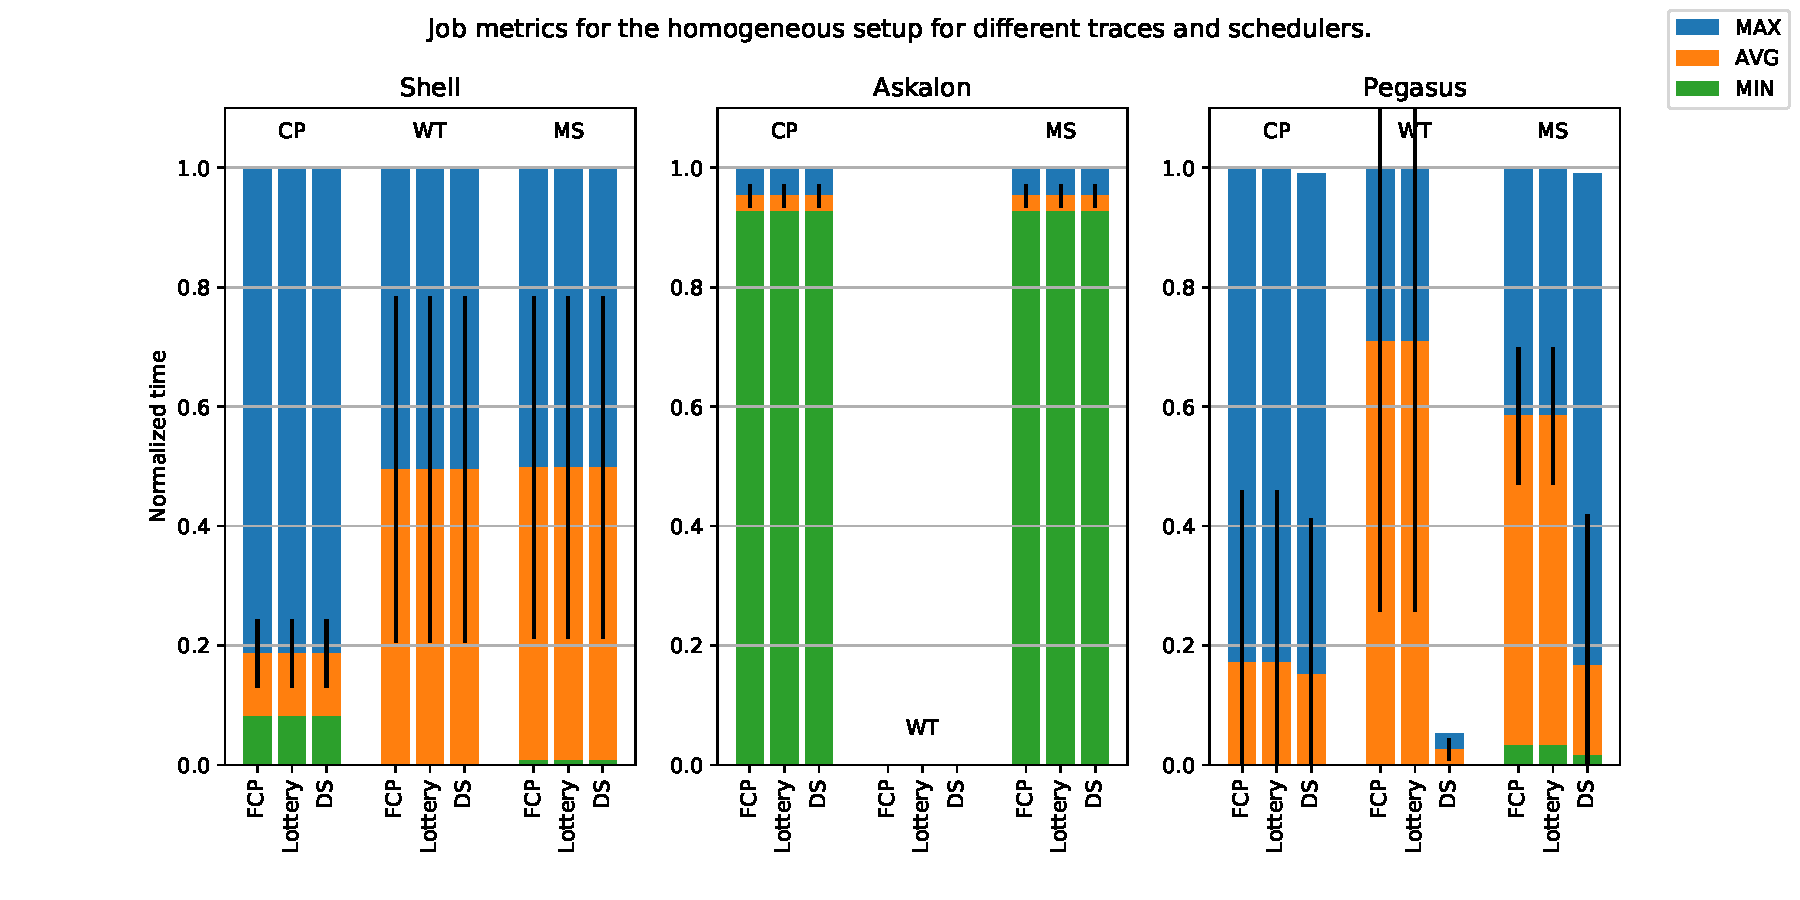
\includegraphics[width=.8\textwidth]{setup_job.pdf}
    
    \caption{Job metrics for the three schedulers for the homogeneous setup for the different traces. Metrics are critical path time (CP), waiting time (WT) and Makespan (MS).}
    \label{fig:setup_job}
\end{figure}

\begin{figure}[H]
    \centering
    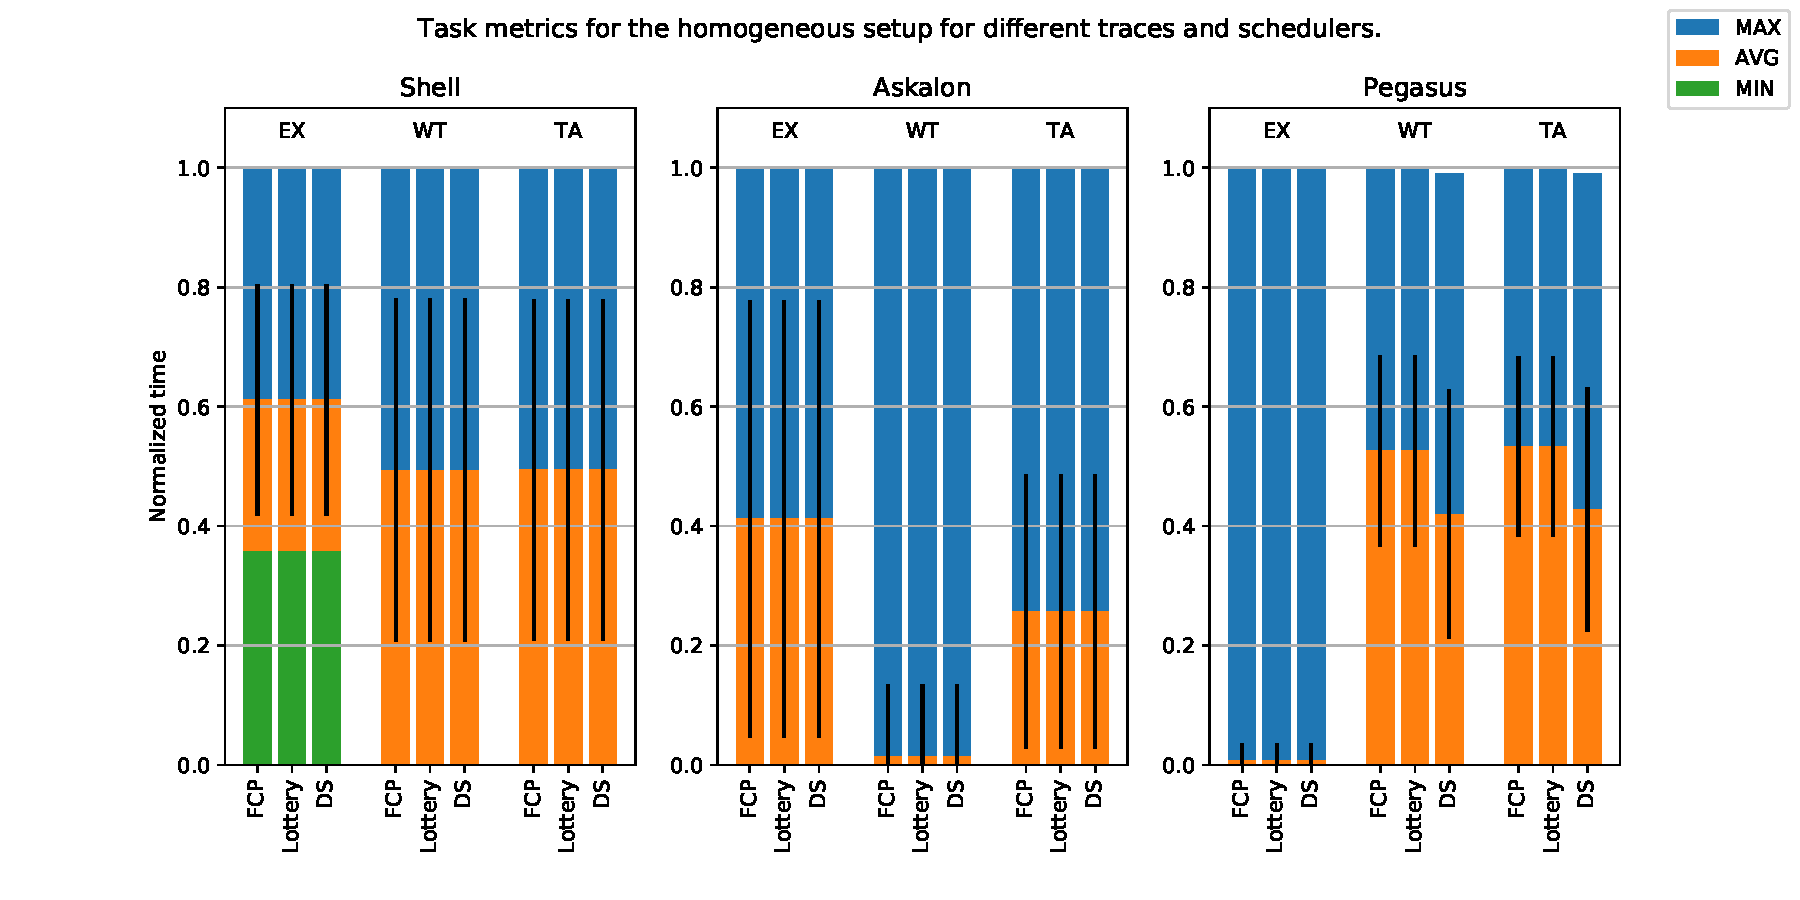
\includegraphics[width=.8\textwidth]{setup_task.pdf}
    \caption{Task metrics for the three schedulers for the homogeneous setup for the different traces. Metrics are execution time (EX), waiting time (WT) and turnaround time (TA).}
    \label{fig:setup_task}
\end{figure}

For the experiments with the homogeneous setup it is clear that the allocation policies have little difference in performance for the Shell and Askalon workloads. With regards to the Pegasus workload, Delay Scheduling performs slightly better in the job metrics CP (Critical Path Time) and MS (Makespan) than both FCP and Lottery. With regards to the WT (Waiting Time), Delay Scheduling sees an enormous increase in performance. When looking at task metrics, all metrics are the same for the Shell and Askalon workloads. With regards, to the Pegasus, we see an improved performance of WT (Waiting Time) and TA (Turnaround Time) for Delay Scheduling, while EX (Execution Time) stays the same for all policies. 
%% Heterogeneous setup %%
\begin{figure}[H]
    \centering
    \centerline{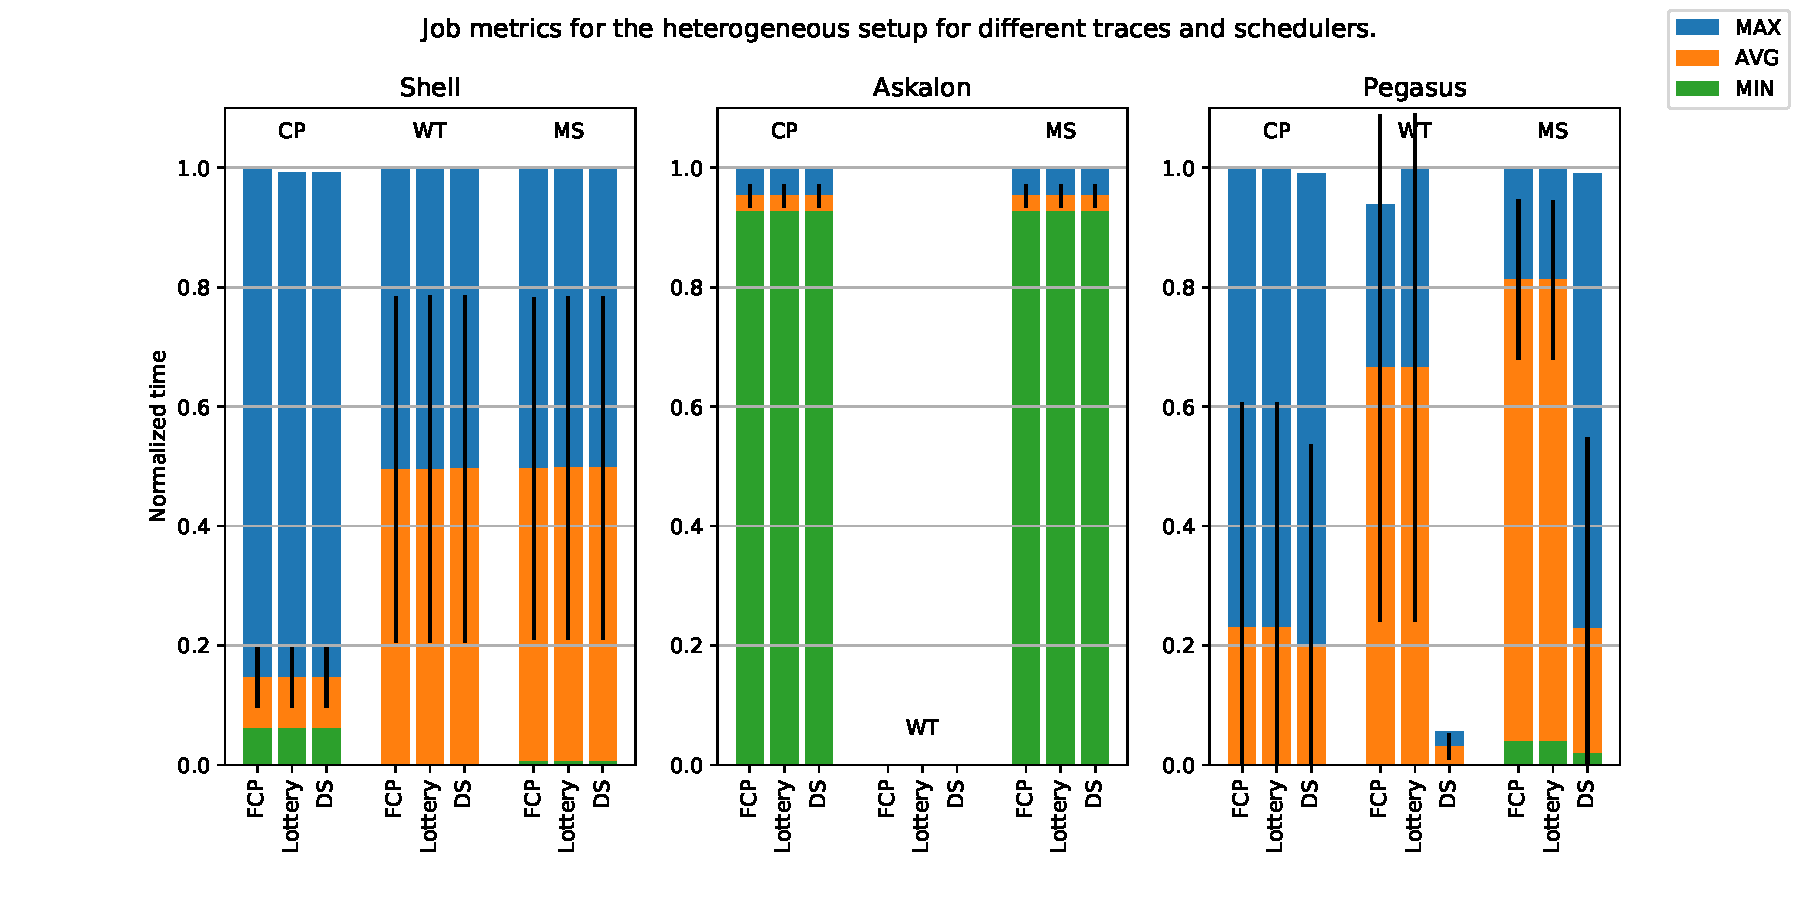
\includegraphics[width=.8\textwidth]{setup-heterogeneous_job.pdf}}
    \caption{Job metrics for the three schedulers for the heterogeneous setup for the different traces. Metrics are critical path time (CP), waiting time (WT) and Makespan (MS).}
    \label{fig:setup-heterogeneous_job}
\end{figure}

\begin{figure}[H]
    \centering
    \centerline{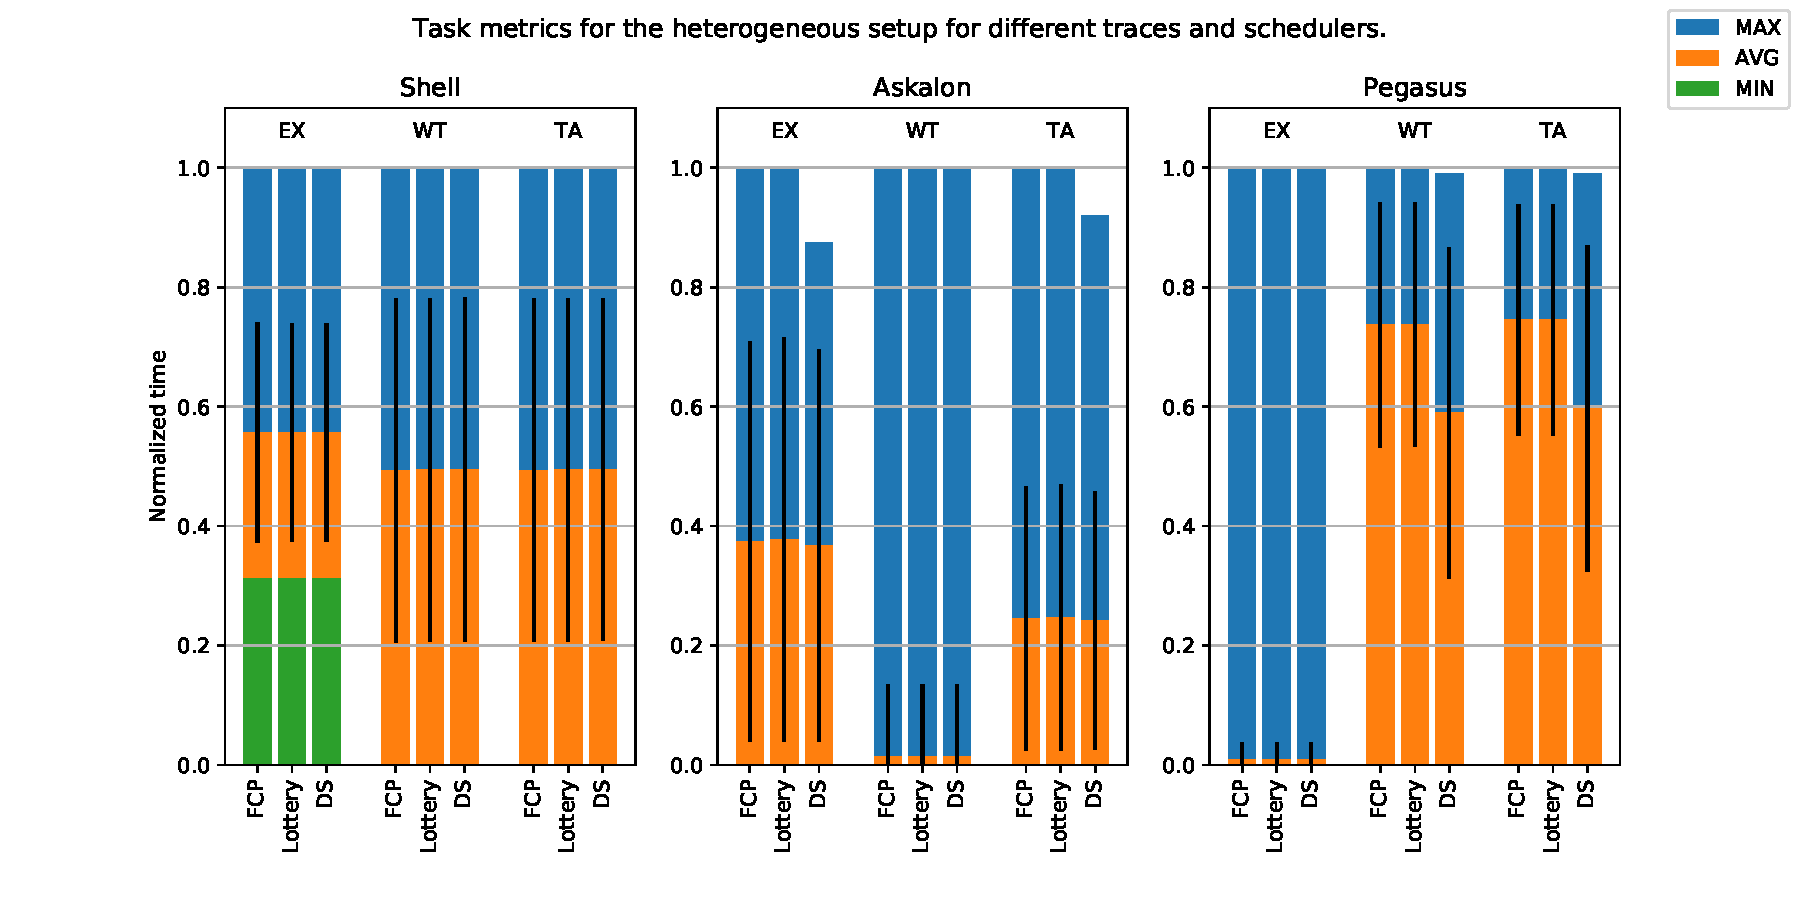
\includegraphics[width=.8\textwidth]{setup-heterogeneous_task.pdf}}
    \caption{Task metrics for the three schedulers for the heterogeneous setup for the different traces. Metrics are execution time (EX), waiting time (WT) and turnaround time (TA).}
    \label{fig:setup-heterogeneous_task}
\end{figure}

When looking at the first two workloads, we see similar results compared with the heterogeneous setup. All job metrics are basically the same. When looking at the Pegasus workload, we see a great performance increase for Delay Scheduling compared to the two other algorithms. The same behaviour is seem of the task metrics. However, the difference in performance is less significant here. 

%% Distributed setup %%
\begin{figure}[H]
    \centering
    \centerline{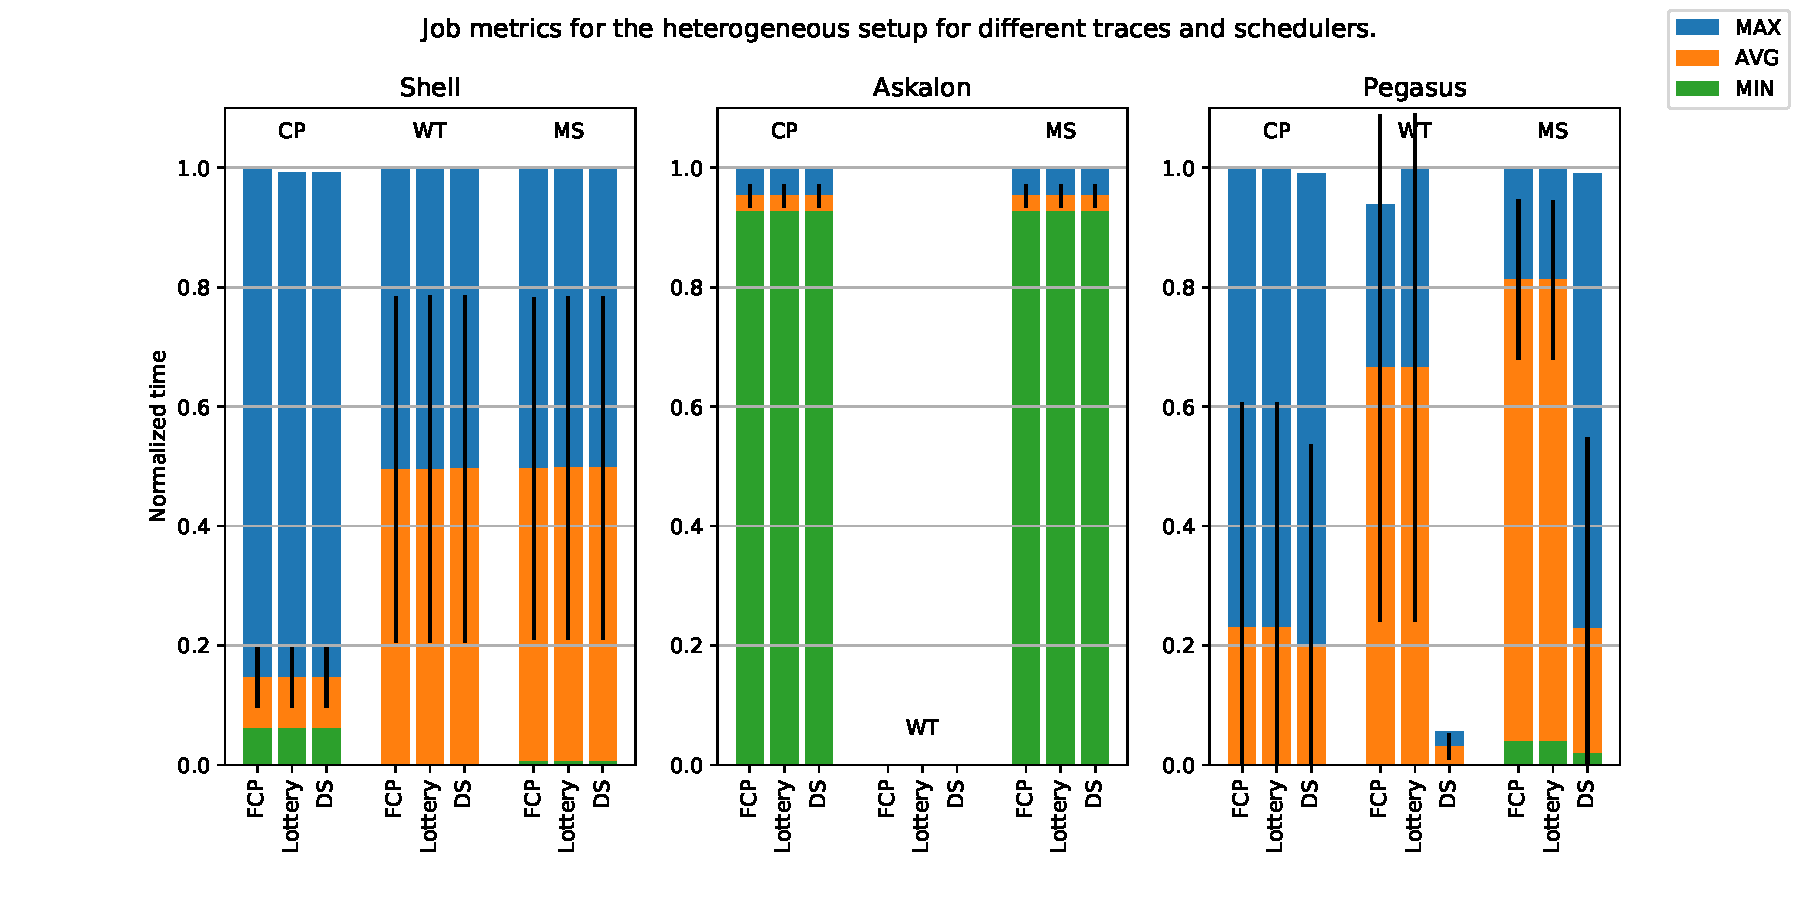
\includegraphics[width=.8\textwidth]{setup-heterogeneous_job.pdf}}
    \caption{Job metrics for the three schedulers for the distributed setup for the different traces. Metrics are critical path time (CP), waiting time (WT) and Makespan (MS).}
    \label{fig:setup-distributed_job}
\end{figure}

\begin{figure}[H]
    \centering
    \centerline{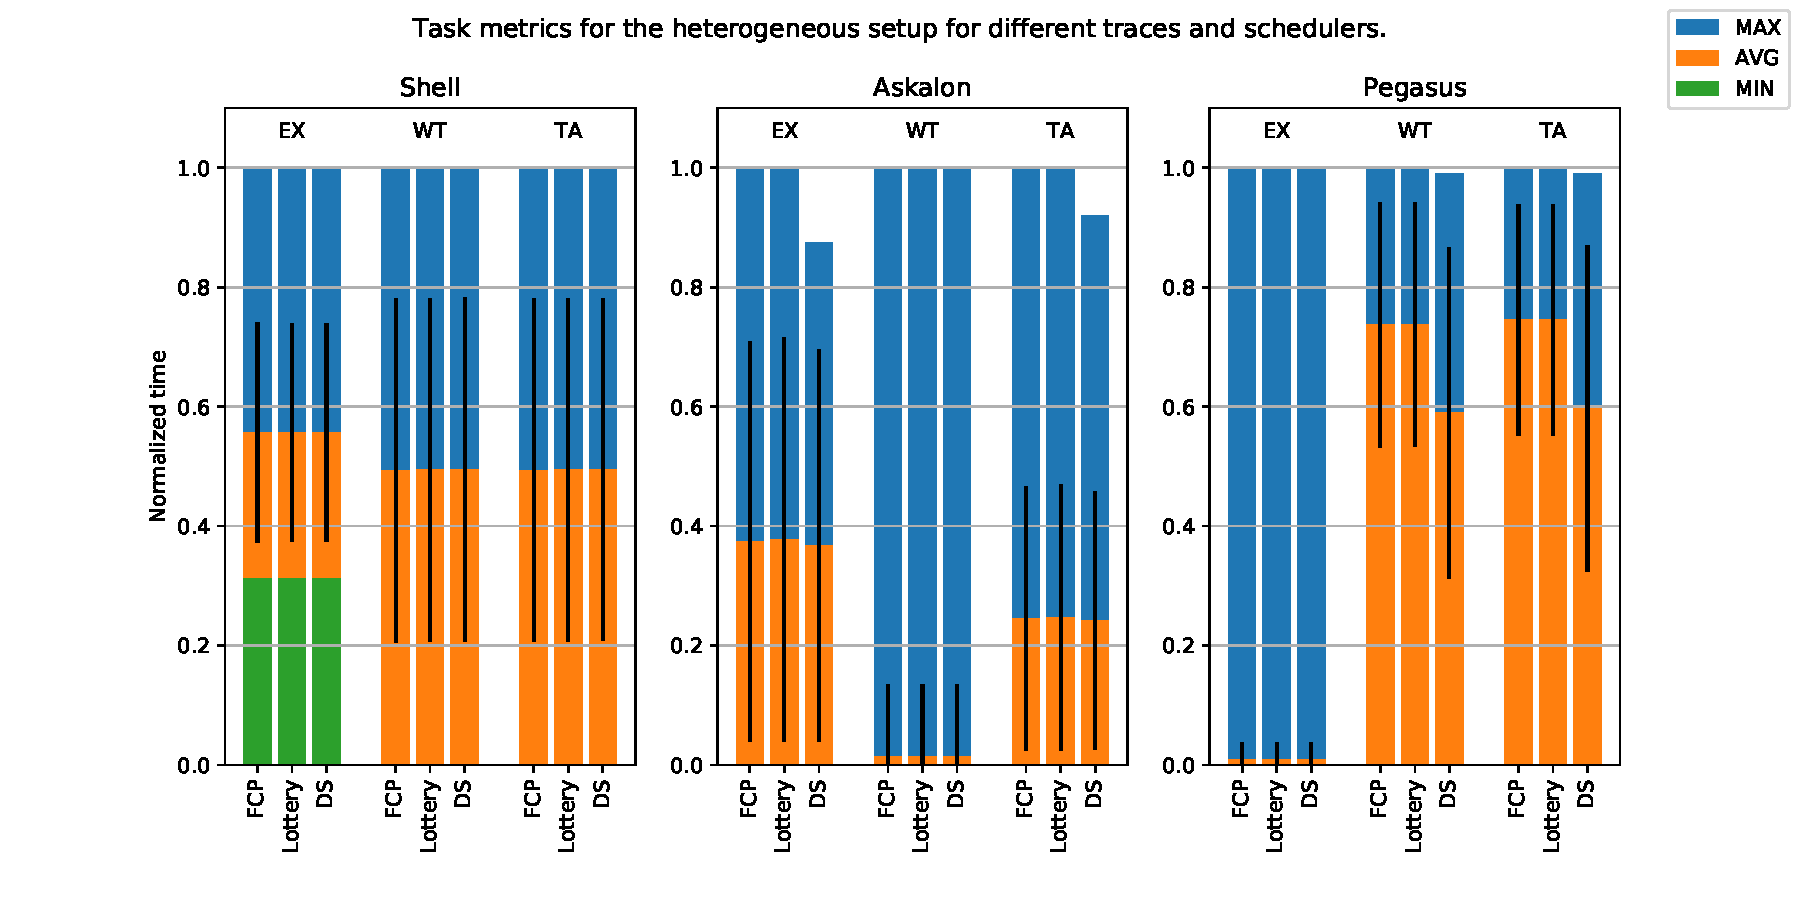
\includegraphics[width=.8\textwidth]{setup-heterogeneous_task.pdf}}
    \caption{Task metrics for the three schedulers for the distributed setup for the different traces. Metrics are execution time (EX), waiting time (WT) and turnaround time (TA).}
    \label{fig:setup-distributed_task}
\end{figure}

With regards to the distributed setup of the environment. The results for the job metrics and the task metrics show the same behaviour as the previous two setups. Specifically, for the Shell and Askalon workloads, all metrics are the same. For the Pegasus workload, Delay Scheduling sees an improvement in all job and task metrics. 

\FloatBarrier

\section{Conclusion}
The performance of FCP, Lottery, and Delay Scheduling are mostly very similar in all settings. Where there a was a measurable difference, Delay Scheduling seemed to function best. The measurable differences in performance were mostly visible while using the Pegasus workload. Taking into account that the Pegasus workflow is a smaller workflow with more heterogeneous jobs, which could mean that there are more tasks within that workload that consist of tasks with dependencies, leading to delay scheduling's scheduling strength.
Overall there were not enough difference in performance between the algorithms on the tested workflows to conclude anything meaningful about their differences.


\section{Discussion}

For future work it would be interesting to test the system with traces that have different resource requirements per task. While these traces were available on the workflow trace archive, they were too large to be ran by our machines in a reasonable time period and attempts to make them smaller unfortunately failed. Further investigation into this approach might allow the testing of these kinds of traces. Furthermore we examined some other schedulers that did not end up in this report. Especially Greedy-Ant scheduling \cite{xiang2017greedy}
seemed like it would perform well, however we could not get it to work in the current environment. More development time could be invested here to implement the algorithm properly.
Lastly an extension of the available machine components in OpenDC for the different setups could be interesting to allow for better testing of the different (theoretical) strong points of the algorithms.

\newpage

\printbibliography

\begin{appendices}
\begin{table}[ht]
\caption{Time table for time spent on various parts of the lab assignment}
\begin{small}
\begin{tabular}{ | l | l | l | l | }
\hline
Date & Person & Type of Time Spent & Activity & Hours \   \\ \hline
13-11-19 & Everybody & think-time & Defining (N)FR Requirements and preparing the meeting on the 14th & 1.0 \\ \hline
14-11-19 & Daan, Kaan, Mike & think-time & Meet with supervisor. (N)FR, report requirements etc & 1.0   \\ \hline
15-11-19 & Mike & write-time & Creating this table & 0.25\   \\ \hline
19-11-19 & Everybody & think-time & Reading up on scheduling policies & 2.5   \\ \hline
21-11-19 & Everybody & think-time & Studying specific policies to decide which to implement & 4.0  \\ \hline
26-11-19 & Daan & dev-time & Working on getting OpenDC to work etc. & 2.5   \\ \hline
27-11-19 & Willemijn \& Mike & wasted-time & Implementing greedy ant & 7.0   \\ \hline
43788.0 & Willemijn \& Mike & think-time & Finding an alternative for greedy ant & 3.0   \\ \hline
28-11-19 & Daan & dev-time & Creating execution and testing scripts  & 2.5 \\ \hline
43818.0 & Kaan & dev-time & Implementing Fast Critical Path & 12.0  \\ \hline
43818.0 & Sander & dev-time & Implementing Lottery Scheduling & 12.0  \\ \hline
43818.0 & Mike & dev-time & Implementing Delay Scheduling & 16.0  \\ \hline
15-12-19 & Daan & xp-time & Working on experiments and plotting and writing the report & 5.0   \\ \hline
16-12-19 & Daan & analysis-time & Finishing experiments and adding discussion to report & 7.0   \\ \hline
18-12-19 & Everybody & write-time & Writing report & 4.0   \\ \hline
19-12-19 & Everybody & write-time & Writing report & 4.0   \\ \hline
20-12-10 & Everybody & write-time & Improving report & 3.0\   \\ \hline
\end{tabular}
\end{small}
\end{table}
\end{appendices}

\end{document}